% !TEX root = Projektdokumentation.tex
\section{Anhang}
\subsection{Detaillierte Zeitplanung}
\label{app:Zeitplanung}

\tabelleAnhang{ZeitplanungKomplett}

\subsection{tt\_content.php}
\label{tt_content.php}

\begin{lstlisting}[language=json,firstnumber=1]
<?php declare(strict_types=1);

defined('TYPO3_MODE') || die();

// static TypoScript
(static function () {
    \TYPO3\CMS\Core\Utility\ExtensionManagementUtility::addPlugin(
        array(
            'LLL:EXT:bal_skeleton/Resources/Private/Language/Tca.xlf:bal_column.wizard.title',
            'tx_bal_column',
            'EXT:bal_skeleton/Resources/Public/Icons/ContentElements/stage.png'
        ),
        'CType',
        'bal_skeleton'
    );
    $temporaryColumn = array(
        'tx_bal_column_color' => array (
            'exclude' => 1,
            'label' => 'LLL:EXT:bal_skeleton/Resources/Private/Language/Tca.xlf:bal_column.color.title',
            'config' => array (
                'type' => 'input',
                'renderType' => 'colorpicker',
                'size' => 10,
            )
        ),
    );

    \TYPO3\CMS\Core\Utility\ExtensionManagementUtility::addTCAcolumns(
        'tt_content',
        $temporaryColumn
    );

    $GLOBALS['TCA']['tt_content']['types']['tx_bal_column'] = array(
        'showitem' => '
            --palette--;LLL:EXT:frontend/Resources/Private/Language/locallang_ttc.xml:palette.general;general,
            tx_bal_column_color,
    ');
})();
\end{lstlisting}

\subsection{ext\_localconf.php}
\label{ext_localconf.php}

\begin{lstlisting}[language=json,firstnumber=1]
<?php
defined('TYPO3_MODE') || die('Access denied.');

use TYPO3\CMS\Extbase\Utility\ExtensionUtility;

call_user_func(
    function () {
        // wizards
        \TYPO3\CMS\Core\Utility\ExtensionManagementUtility::addPageTSConfig(
            'mod.wizards.newContentElement.wizardItems.common {
           elements {
              tx_bal_column {
                 iconIdentifier = bal_column
                 title = LLL:EXT:bal_skeleton/Resources/Private/Language/Tca.xlf:bal_column.wizard.title
                 description = LLL:EXT:bal_skeleton/Resources/Private/Language/Tca.xlf:bal_column.wizard.description
                 tt_content_defValues {
                    CType = tx_bal_column
                 }
              }
           }
           show := addToList(tx_bal_column)
        }'
        );

        $iconRegistry = \TYPO3\CMS\Core\Utility\GeneralUtility::makeInstance(\TYPO3\CMS\Core\Imaging\IconRegistry::class);

        $iconRegistry->registerIcon(
            'bal_column',
            \TYPO3\CMS\Core\Imaging\IconProvider\SvgIconProvider::class,
            ['source' => 'EXT:bal_skeleton/Resources/Public/Icons/ContentElements/stage.svg']
        );
   }
);
\end{lstlisting}

\subsection{[...slug].vue}
\label{[...slug].vue}

\begin{lstlisting}[language=json,firstnumber=1]
<script setup lang="ts">
  const runtimeConfig = useRuntimeConfig()
  const route = useRoute();
  const { data } = await useAsyncData(
      "pageData",
    () => $fetch(runtimeConfig.typo3 + route.fullPath),
    {initialCache: false}
  )
  let breadcrumbs = data.value.breadcrumbs;
  let content = data.value.content.colPos0;
  let mainNavigation = data.value.page.navigation.main;
  let metaData = data.value.meta;

  useHead({
    title: metaData.title,
    meta: [
      { name: 'description', content: metaData.description ? metaData.description : '' }
    ]
  })

</script>
<template>
     <div>
          <template v-if="mainNavigation"><Navigation :typo3-navigation="mainNavigation"></Navigation></template>
          <div class="container mx-auto xl">
            <template v-if="breadcrumbs"><Breadcrumbs :typo3breadcrumbs="breadcrumbs"></Breadcrumbs></template>
            <template v-if="content"><TypoView :typo3-content="content"></TypoView></template>
            <h3 v-else>Noch kein Content gepflegt!</h3>
          </div>
     </div>
</template>
\end{lstlisting}

\subsection{navigation.ts}
\label{navigation.ts}

\begin{lstlisting}[language=json,firstnumber=1]
export const useNavigation = () => {
    const fullNavList = useState('fullNavList', () => []);
    const navigationOpened = useState('navigationOpened', () => false);
    const currentNavList = useState('currentNavList', () => []);
    const previousNavItem:{value: navigationItem | Record<string, never>} = useState('previousNavItem');
    const router = useRouter();
    
    const open = (navItem: navigationItem) => {
        if (!navItem.hasSubpages) {
            router.push(navItem.link)
        } else {
            previousNavItem.value = navItem;
            currentNavList.value = navItem.children;
            navigationOpened.value = true;  
        } 
    }
    const close = () => {
        navigationOpened.value = false;
    }
    const navigate = (navItem: navigationItem) => {
        if (!navItem.hasSubpages) {
            close();
            router.push(navItem.link)
        }
        else {
            previousNavItem.value = navItem;
            currentNavList.value = navItem.children;
        }
    }
    const back = () => {
        const parent = findParent(fullNavList.value, previousNavItem.value.uid);
        if (parent && parent.children) {
            previousNavItem.value = parent;
            currentNavList.value = parent.children;
        } else {
            previousNavItem.value = {};
            currentNavList.value = fullNavList.value;
        }
    }
    const findParent = (nav: navigationItem[], id: number, potentialParentNav?: navigationItem) => {
        let parent: navigationItem;
        for (let index = 0; index < nav.length; index++) {
            const item = nav[index];
            if (item.uid === id) {
                parent = potentialParentNav;
                break;
            } 
            else {
                if (item.children && item.children.length > 0) {
                        parent = findParent(item.children, id, item);
                        if (parent) {
                            break;
                        }
                    }
                }
        }
        return parent;
    }
    return {fullNavList, navigationOpened, open, close, currentNavList, previousNavItem, navigate, back};
}
\end{lstlisting}

\subsection{SlideMenu.vue}
\label{SlideMenu.vue}

\begin{lstlisting}[language=json,firstnumber=1]
<script setup>
    const {fullNavList, navigationOpened, close, currentNavList, previousNavItem, navigate, back} = useNavigation();
</script>
<template>
    <div class="slidemenu-container" :class="{'active' : navigationOpened}">
        <div class="flex">
            <div class="text-xl font-bold cursor-pointer" v-if="fullNavList != currentNavList" @click="back()">back</div>
            <div class="text-xl font-bold pl-6 grow" v-if="previousNavItem">
                <NuxtLink :to="previousNavItem.link" @click="close()">{{previousNavItem.title}}</NuxtLink>
            </div>
            <div class="text-xl font-bold cursor-pointer" @click="close()">X</div>
        </div>
        <hr>
        <div class="navbar">
            <div class="btn btn-ghost normal-case text-xl" v-for="navItem in currentNavList" :key="navItem.uid" @click="navigate(navItem)">
                {{navItem.title}}
            </div>
        </div>
    </div>
</template>
<style>
    .slidemenu-container {
        position: absolute;
        height: 100vh;
        width: 0px;
        transition: width 0.5s;
        background: white;
        overflow-x: hidden;
        z-index: 100;
    }
    .slidemenu-container.active {
        width: 400px;
    }
</style>
\end{lstlisting}

\subsection{Datenbankmodell}
\label{app:Datenbankmodell}
ER-Modelle kann man auch direkt mit \LaTeX{} zeichnen, siehe \zB \url{http://www.texample.net/tikz/examples/entity-relationship-diagram/}.
\begin{figure}[htb]
\centering
\includegraphicsKeepAspectRatio{database.pdf}{1}
\caption{Datenbankmodell}
\end{figure}
\clearpage
\input{Anhang/AnhangMenü.tex}
\clearpage
\subsection{Oberflächenentwürfe}
\label{app:Entwuerfe}
\begin{figure}[htb]
\centering
\includegraphicsKeepAspectRatio{MockupModules.pdf}{0.7}
\caption{Liste der Module mit Filtermöglichkeiten}
\end{figure}

\begin{figure}[htb]
\centering
\includegraphicsKeepAspectRatio{MockupModul.pdf}{0.7}
\caption{Anzeige der Übersichtsseite einzelner Module}
\end{figure}

\begin{figure}[htb]
\centering
\includegraphicsKeepAspectRatio{MockupTag.pdf}{0.7}
\caption{Anzeige und Filterung der Module nach Tags}
\end{figure}

\clearpage
\subsection{Screenshots der Anwendung}
\label{Screenshots}
\begin{figure}[htb]
\centering
\includegraphicsKeepAspectRatio{tagliste.pdf}{1}
\caption{Anzeige und Filterung der Module nach Tags}
\end{figure}
\clearpage
\begin{figure}[htb]
\centering
\includegraphicsKeepAspectRatio{modulliste.pdf}{1}
\caption{Liste der Module mit Filtermöglichkeiten}
\end{figure}
\clearpage

\subsection{Entwicklerdokumentation}
\label{app:Doc}
\begin{center}
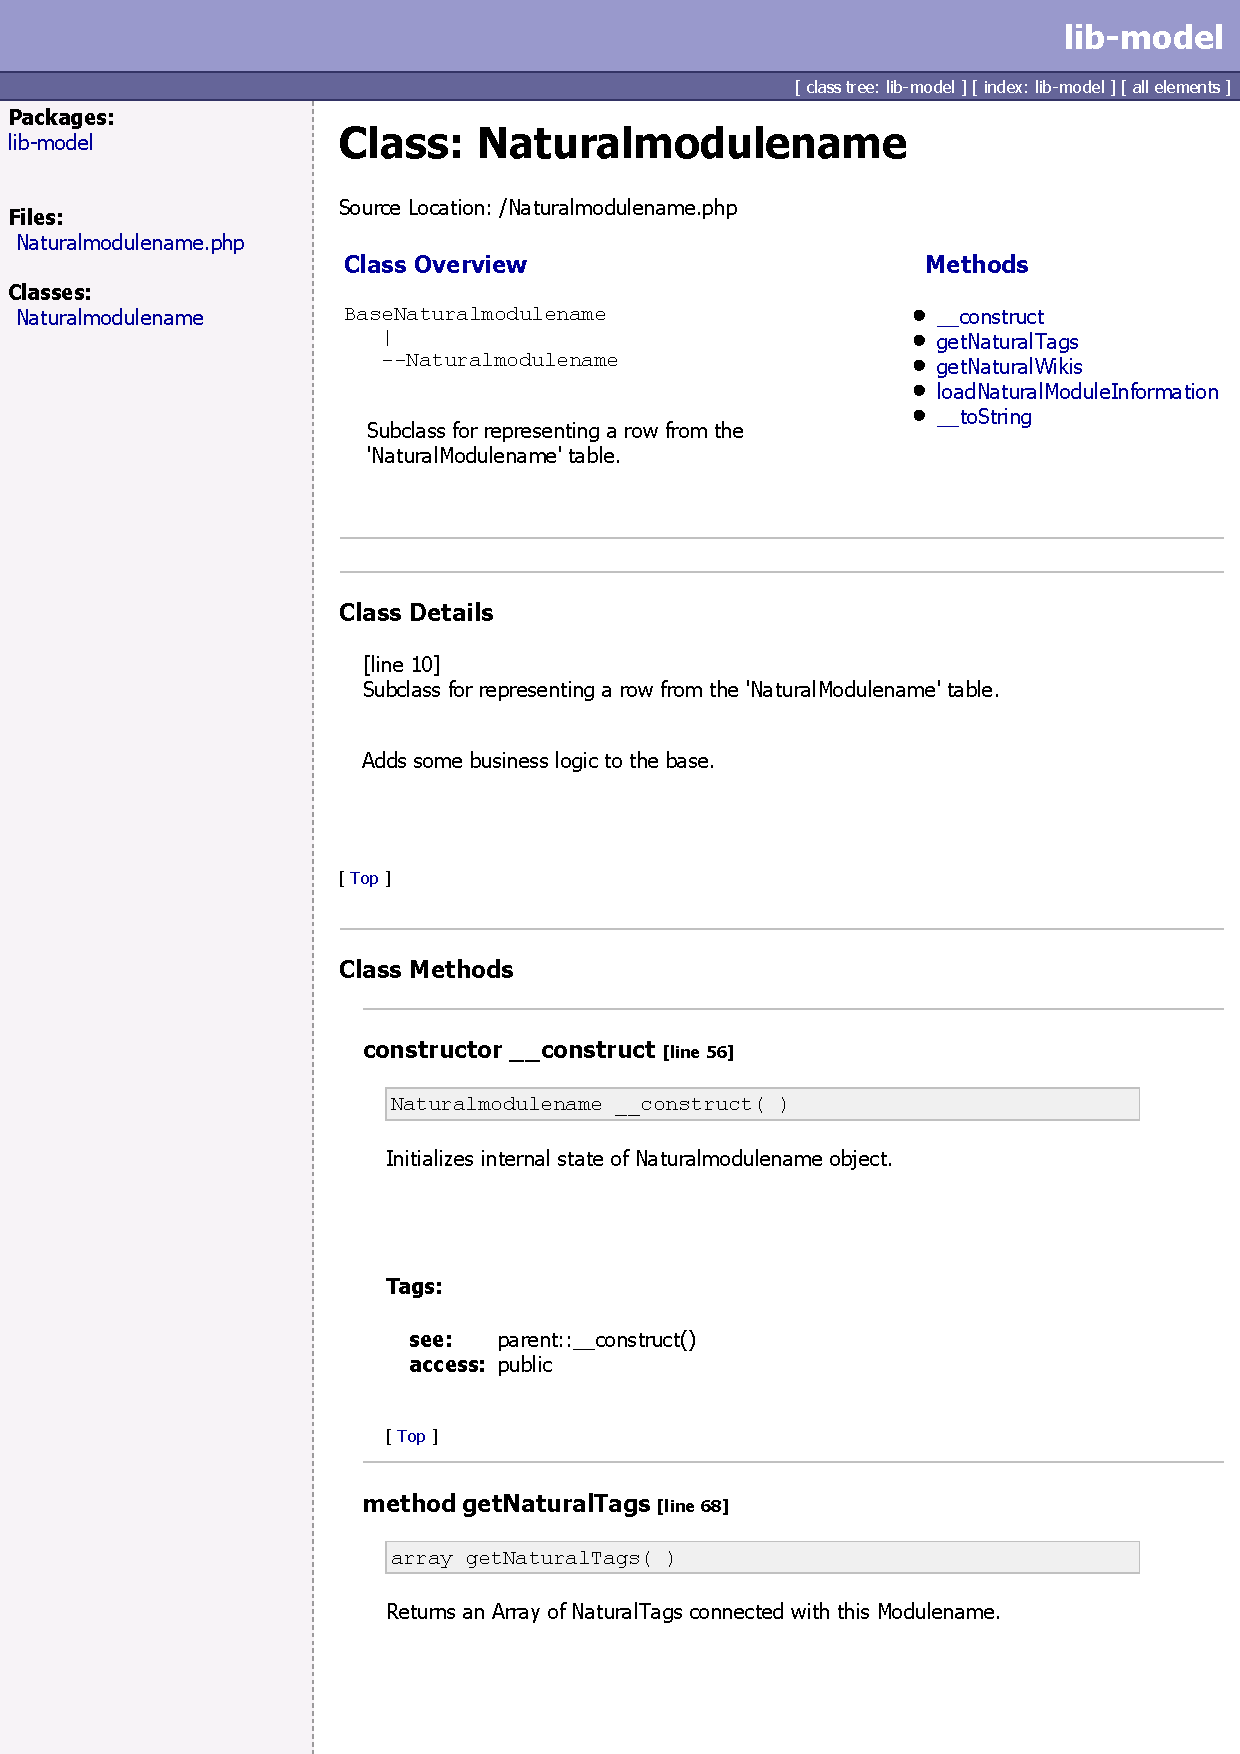
\includegraphics[page=1, width=0.9\textwidth]{doc.pdf}

\includegraphics[page=2, width=0.9\textwidth]{doc.pdf}
\end{center}

\clearpage
\subsection{Testfall und sein Aufruf auf der Konsole}
\label{app:Test}
\lstinputlisting[language=php, caption={Testfall in PHP}]{Listings/tests.php}
\clearpage
\begin{figure}[htb]
\centering
\includegraphicsKeepAspectRatio{testcase.jpg}{1}
\caption{Aufruf des Testfalls auf der Konsole}
\end{figure}


\subsection{Klasse: ComparedNaturalModuleInformation}
\label{app:CNMI}
Kommentare und simple Getter/Setter werden nicht angezeigt.
\lstinputlisting[language=php, caption={Klasse: ComparedNaturalModuleInformation}]{Listings/cnmi.php}
\clearpage

\subsection{Klassendiagramm}
\label{app:Klassendiagramm}
Klassendiagramme und weitere \acs{UML}-Diagramme kann man auch direkt mit \LaTeX{} zeichnen, siehe \zB \url{http://metauml.sourceforge.net/old/class-diagram.html}.
\begin{figure}[htb]
\centering
\includegraphicsKeepAspectRatio{Klassendiagramm.pdf}{1}
\caption{Klassendiagramm}
\end{figure}
\clearpage

\subsection{Benutzerdokumentation}
\label{app:BenutzerDoku}
Ausschnitt aus der Benutzerdokumentation:

\begin{table}[htb]
\begin{tabularx}{\textwidth}{cXX}
\rowcolor{heading}\textbf{Symbol} & \textbf{Bedeutung global} & \textbf{Bedeutung einzeln} \\
\includegraphicstotab[]{weather-clear.png} & Alle Module weisen den gleichen Stand auf. & Das Modul ist auf dem gleichen Stand wie das Modul auf der vorherigen Umgebung. \\
\rowcolor{odd}\includegraphicstotab[]{weather-clear-night.png} & Es existieren keine Module (fachlich nicht möglich). & Weder auf der aktuellen noch auf der vorherigen Umgebung sind Module angelegt. Es kann also auch nichts übertragen werden. \\
\includegraphicstotab[]{weather-few-clouds-night.png} & Ein Modul muss durch das Übertragen von der vorherigen Umgebung erstellt werden. & Das Modul der vorherigen Umgebung kann übertragen werden, auf dieser Umgebung ist noch kein Modul vorhanden. \\
\rowcolor{odd}\includegraphicstotab[]{weather-few-clouds.png} & Auf einer vorherigen Umgebung gibt es ein Modul, welches übertragen werden kann, um das nächste zu aktualisieren. & Das Modul der vorherigen Umgebung kann übertragen werden um dieses zu aktualisieren. \\
\includegraphicstotab[]{weather-storm.png} & Ein Modul auf einer Umgebung wurde entgegen des Entwicklungsprozesses gespeichert. & Das aktuelle Modul ist neuer als das Modul auf der vorherigen Umgebung oder die vorherige Umgebung wurde übersprungen. \\
\end{tabularx}
\end{table}



